\subsubsection{System Overview}
\label{sec:system-overview}

\begin{figure}[ht]
    \centering
    \makebox[\linewidth][c]{%
        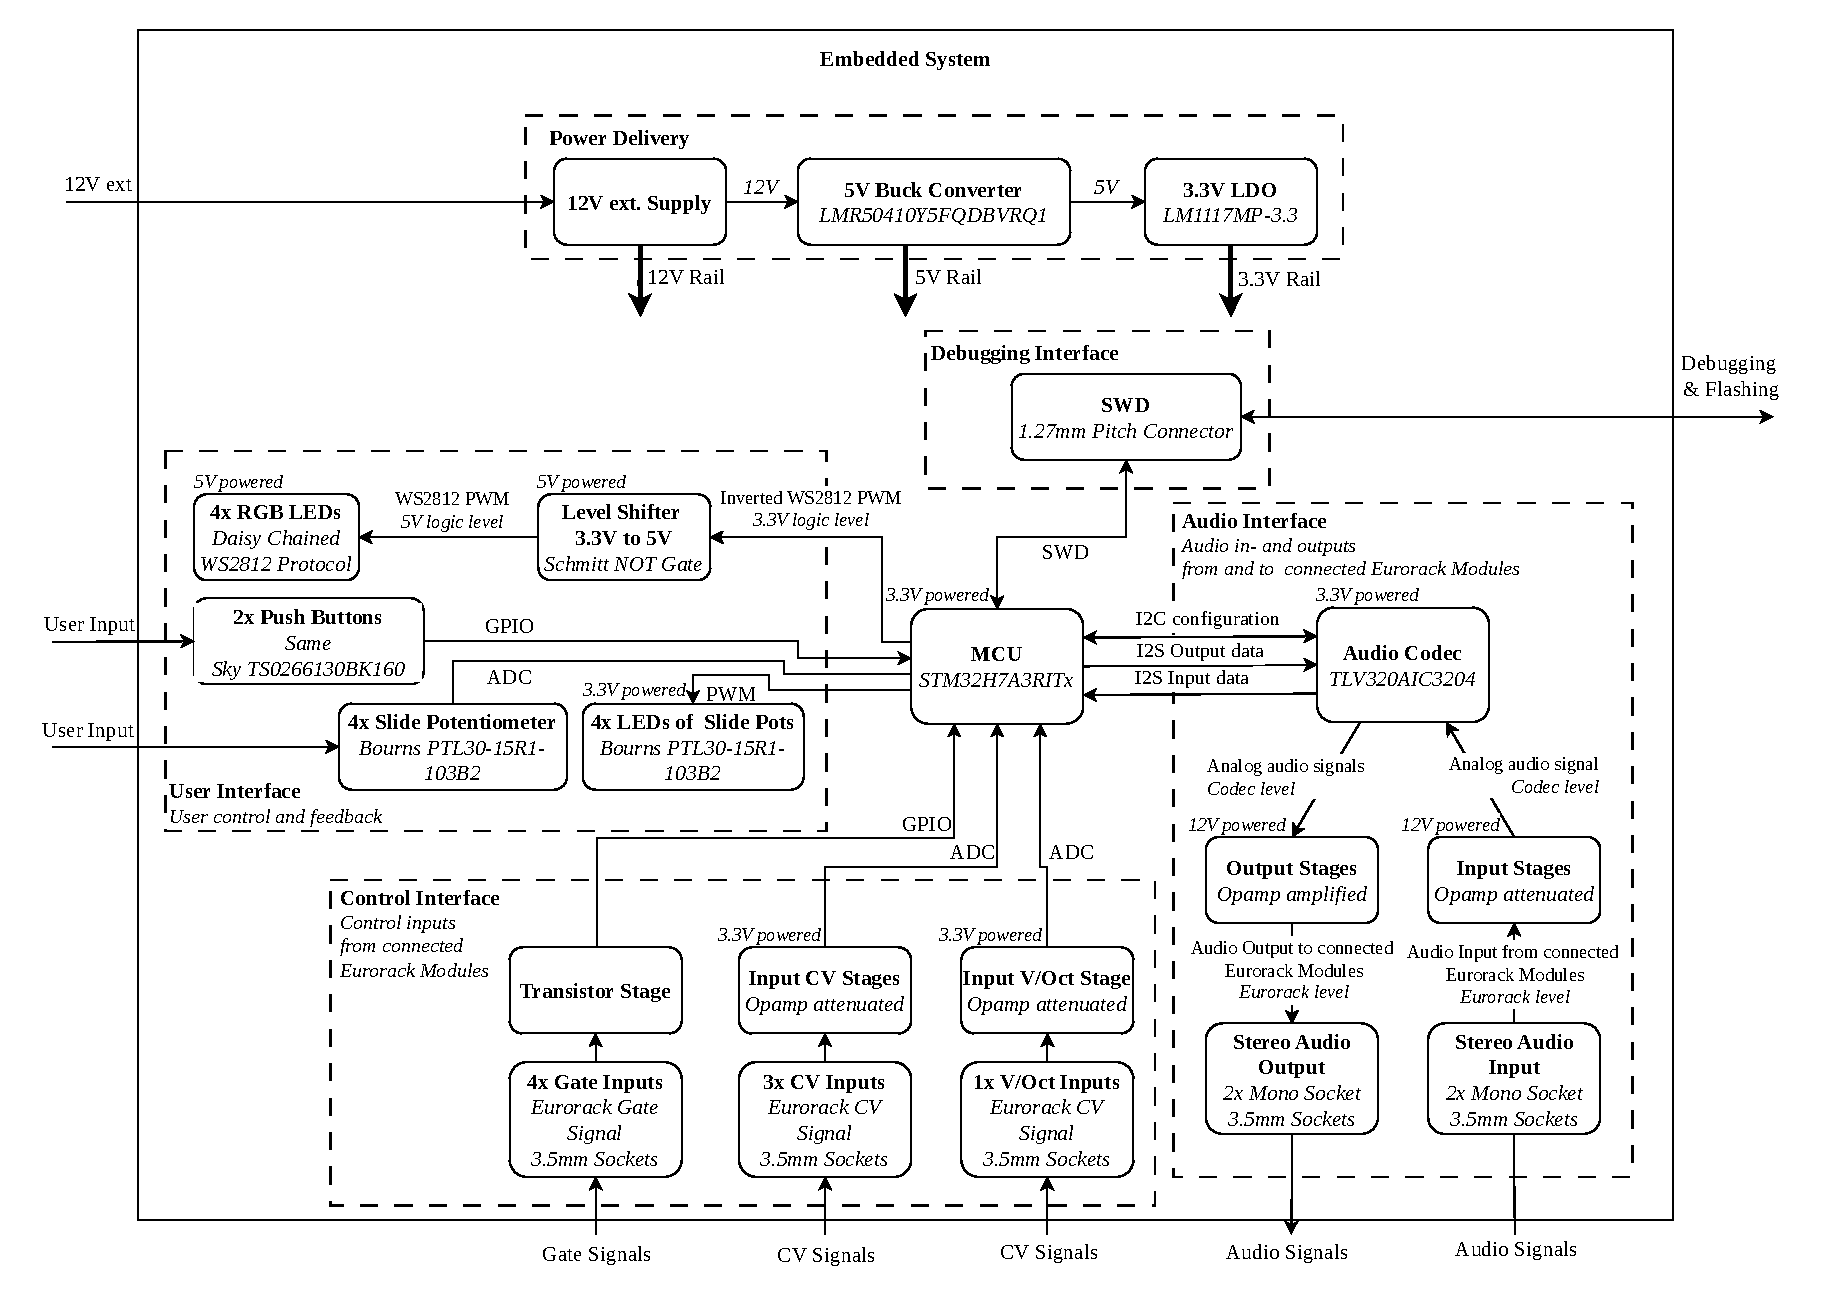
\includegraphics[width=1.1\linewidth]{../images/hardware_design/componentdiagram_hardware.drawio.pdf}
    }
    \caption{Hardware component diagram}
    \label{fig:block-diagram}
\end{figure}
\FloatBarrier


Figure~\ref{fig:block-diagram} shows the top-level block diagram of the embedded system.
The design is organised into five functional domains: power delivery, the microcontroller 
unit (MCU), user interface, control interface, and audio interface.

\paragraph{Power Delivery}
The external Eurorack \qty{12}{V} supply feeds a \textit{LMR50410Y5FQDBVRQ1}\cite{Lmr50410q1} buck converter, which steps the voltage down to \qty{5}{V}. 
A subsequent \textit{LM1117MP-3.3}\cite{Lm1117} LDO regulator provides the \qty{3.3}{V} rail required by the MCU and codec. 
The \qty{12}{V} rail is retained for the output and input opamp stages, which require higher voltage headroom for Eurorack-level signals.

\paragraph{Microcontroller}
The central processing element is an \textit{STM32H7A3RITx}\cite{stmicroelectronicsStm32h7a3riDatasheet}, connected to all 
subsystems. 
It communicates with the audio codec via I\textsuperscript{2}S for audio 
data and I\textsuperscript{2}C for configuration. 
GPIO and ADC peripherals interface with the user controls, and additional ADC inputs handle the control voltage and V/Oct signals. 
A \qty{1.27}{mm} pitch SWD connector provides debugging and flashing.

\paragraph{User Interface}
Four slide potentiometers (\textit{Bourns PTL30-15R1-103B2}\cite{PTLDatasheet}) are read by the MCU ADC and provide continuous parameter control. 
Two push buttons (\textit{SameSky TS02} \cite{Ts02Datasheet}) are connected as GPIO inputs. 
Four WS2812 RGB LEDs, daisy-chained and driven via a PWM signal, provide visual feedback. Because the WS2812 protocol requires \qty{5}{V} logic, a level shifter based on a Schmitt NOT gate (\textit{TI SN74AHCT1G14} \cite{Sn74ahct1g14}) converts the \qty{3.3}{V} MCU output. 
The slide potentiometers also carry individual LEDs driven by PWM. For the current hardware revision these are not usable due to an error in symbol/footprint creation.

\paragraph{Control Interface}
Three classes of Eurorack control signals are accepted via \qty{3.5}{mm} sockets (\textit{QingPu WQP-PJ398SM} \cite{WQP-PJ398SM}): 
four gate inputs, three CV inputs, and one V/Oct input. 
The gate signals are conditioned by a transistor stage (\textit{MMBT3904} \cite{2N3904MMBT3904PZT39042002a}) before reaching the MCU GPIO. 
The CV and V/Oct signals pass through opamp (\textit{TI OPA2322} \cite{opa2322Datasheet}) attenuation stages before being read by the MCU ADC.

\paragraph{Audio Interface}
Stereo audio input and output are provided via pairs of \qty{3.5}{mm} mono sockets (\textit{QingPu WQP-PJ398SM} \cite{WQP-PJ398SM}) at Eurorack signal levels. 
On the input path, an opamp attenuation stage scales the incoming signal to codec level before it reaches the audio codec (\textit{TI TLV320AIC3204} \cite{texasinstrumentsTlv320aic3204Datasheet}). 
On the output path, the codec signal is amplified by an opamp stage back to Eurorack level. 
The codec performs all analogue-to-digital and digital-to-analogue conversion, 
exchanging audio data with the STM32H7 over I\textsuperscript{2}S.

%The STM32H7 generates a master clock (MCLK) of \qty{12.288}{MHz} 
%($256 \times \qty{48}{kHz}$) via PLL2, which the TLV320AIC3204 uses as its reference to derive BCLK and LRCK internally, operating as an 
%I\textsuperscript{2}S slave.